\fancyhead[L]{Guide Utilisateur}
\fancyhead[C]{Overlay de sélection d'équipe}

\section{Overlay de sélection d'équipe}
\subsection{Qu'est-ce que l'overlay de sélection d'équipe ?}
Palantir va pouvoir vous aider pendant la sélection des équipes en analysant les équipes choisies par les autres joueurs en temps réel et ainsi vous donner la meilleure civilisation à jouer dans cette situation.

\begin{figure}[ht!]
    \begin{center}
        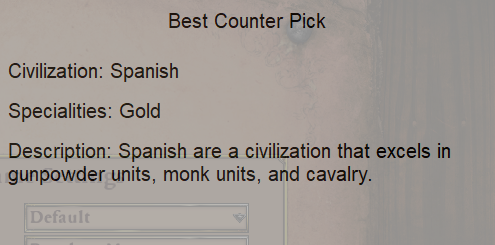
\includegraphics[scale = 1]{team-selection-overlay.png}
    \end{center}
    \caption{Overlay de sélection d'équipe}
\end{figure}

Notez bien que le calcul du meilleur contre se base sur les contres de chaque civilisation inscrite dans le fichier des contres "counters.json".

\subsection{Fichier des contres "counters.json"}
Dans le fichier des contres, vous aurez la possibilité d'ajouter ou de retirer un contre d'une civilisation particulière. Ceci peut être utile lorsqu'une civilisation se fait buff lors d'un patch et qu'elle n'est plus contrée par une certaine civilisation et vice-versa. La structure du fichier est simple et est la suivante:
\begin{minted}{JSON}
{
    "NomDeCivilisation": {
        "counters": [
            "Civilisation1",
            "Civilisation2"
        ]
    }
}
\end{minted}

Les 42 civilisations sont déjà pré-remplie avec des contres qui sont pertinents au moment de la publication de la dernière version de Palantir.